\documentclass[a4paper,12pt]{article}
\usepackage[brazil]{babel}   
\usepackage[utf8]{inputenc}        
\usepackage{epsfig,subfigure, epstopdf}
\usepackage{amssymb,url}
\usepackage{xcolor,tikz,bm,colortbl}
\usepackage{pgfplots}
\usepackage{multirow}
\usepackage{amsmath}
\usepackage{booktabs, comment}
\usepackage{nicealgo}

\begin{document}

\thispagestyle{empty}

\begin{center}
\renewcommand{\baselinestretch}{1}
\end{center}

\vspace*{1cm}

\begin{center}
\textbf{Mestrado Acadêmico IBILCE/São José do Rio Preto\\}
\textbf{Universidade Estadual Paulista ``Júlio de Mesquita Filho"}

\vspace*{1cm}

\renewcommand{\baselinestretch}{2}
\bf {\huge \sc APOSTILA DE TÓPICOS ESPECIAIS: APRENDIZADO DE MÁQUINA}
\renewcommand{\baselinestretch}{1}

\end{center}

\vspace*{2.0cm}

\begin{center}

\large Prof. Dr. Jo\~{a}o Paulo Papa

\vspace*{1.0cm}

\large Contribuinte: Gustavo Henrique de Rosa

\vspace*{1.0cm}

Departamento de Computa\c{c}\~{a}o, Faculdade de Ci\^{e}ncias, Universidade Estadual Paulista J\'ulio de Mesquita Filho\\
Av. Eng. Luiz Edmundo Carrijo Coube, 14-01 - Vargem Limpa, CEP 17033-360 - Bauru - SP.

\end{center}

\vspace*{4cm}

\centerline{\large BAURU}

\vspace*{0.25cm}

\centerline{\large 2016}



\tableofcontents

\newpage

\section{Introdução}
\label{s.introducao}

\begin{center}
\emph{Machine Learning} (mais teórico) x \emph{Pattern Recognition} x \emph{Artificial Intelligence} (área maior, lógica fuzzy)
\end{center}

Podemos considerar o \emph{Machine Learning} e o \emph{Pattern Recognition} como uma inteligência artificial aplicada, isto é, redes neurais, SVM, \emph{Deep Learning}.

\begin{center}
Imagem $\longrightarrow$ Extração de características $\longrightarrow$ Espaço de características	
\end{center}

O conjunto de dados é composto por um conjunto de treinamento, utilizado para aprender e determinar a função separadora do espaço (parâmetros). E também é composto por um conjunto de teste, utilizado em novas amostras e para definir o grupo das mesmas.

\begin{center}
\emph{Machine Learning} $\longrightarrow$ supervisionado (dados rotulados) ou não supervisionado
\end{center}

\subsection{Exemplos de Técnicas}
\label{ss.tecnicas}

\begin{itemize}
	\item SVM - support vector machine: parte do princípio que os dados podem ser separados. O problema se dá quando aumentamos o número de parâmetros, trazendo um maior custo computacional;

	\item Reconhecimento de padrões: o problema é dividido em classificação e regressão (encontrar o fitting, ou seja, a melhor função que modela o problema).	
\end{itemize}

\section{Regressão Linear}
\label{s.linear_regression}

\subsection{Uma Variável (Univariado)}
\label{ss.one_variable}
 
 Suponha que tenhamos o problema de predizer preços de casas, como demonstradas abaixo. A regressão do problema tem por objetivo estimar (predizer) valores reais de saída, dado uma entrada. Considerando o problema mencionado, gostaríamos de estimar o preço de uma casa dado o seu tamanho, isto é, gostaríamos de encontrar a \textbf{linha reta} a qual melhor se adapta aos pontos da base de dados (dados de treinamento).\\
 
  \begin{center}
 	\begin{tikzpicture}[domain=0:3]
  	\begin{axis}[ 
    	xlabel=Tamanho ($10^3$),
    	ylabel={Preço ($10^3$)}
  		] 
    	\addplot[blue, thick] {x}; 
    	\addplot[only marks, red] plot coordinates {
        (0.5,0.5)
        (0.9,1)
        (1, 1)
        (0.8,1.2)
        (1.25, 1.15)
        (1.4, 1.2)
        (1.3, 1.5)
        (1.75, 1.85)
        (2, 2)
        (2.5, 2.3)
        (2.6, 2.8)
        
    };
  	\end{axis}
	\end{tikzpicture}
 \end{center}
 
 \textbf{Exemplo:} Seja $m$ o número de exemplos de treinamento, $x \in \mathbb{R}$ a variável de entrada (características) e $y \in \mathbb{R}$ a variável de saída (objetivo). Então, um treinamento simples de treinamento é denotado por $(x, y)$, sendo o conjunto de treinamento $X$ composto por todas as amostradas de treinamento, isto é, $X = \{(x, y), (x_2, y_2), \dots, (x_m, y_m)\}$. Usualmente, nós possuímos o seguinte fluxo de dados:
 
 \begin{center}
 Dados de treinamento $X \longrightarrow$ Algoritmo de treinamento $\longrightarrow h$ (tamanho da casa) $\longrightarrow$ preço estimado	
 \end{center}

 A função linear pode ser definida como $h_w(x) = w_0 + w_1x$, onde $w_0$ e $w_1$ são os parâmetros do modelo. Suponha que tenhamos os seguintes exemplos:
 
 \begin{center}
 	\begin{tikzpicture}[domain=0:3]
  	\begin{axis}[ 
    	xlabel=$x$,
    	ylabel={$h_w(x) = 1.5 + 0x$}
  		] 
    	\addplot[blue, thick] {1.5 + 0*x}; 
  	\end{axis}
	\end{tikzpicture}
 \end{center}
 
  \begin{center}
 	\begin{tikzpicture}[domain=0:3]
  	\begin{axis}[ 
    	xlabel=$x$,
    	ylabel={$h_w(x) = 0.5x$}
  		] 
    	\addplot[blue, thick] {0.5*x}; 
  	\end{axis}
	\end{tikzpicture}
 \end{center}
 
  \begin{center}
 	\begin{tikzpicture}[domain=0:3]
  	\begin{axis}[ 
    	xlabel=$x$,
    	ylabel={$h_w(x) = 1 + 0.5x$}
  		] 
    	\addplot[blue, thick] {1 + 0.5*x}; 
  	\end{axis}
	\end{tikzpicture}
 \end{center}
 
 Portanto, possuímos diferentes comportamentos envolvendo $h_w(x)$, o qual é chamado de \textbf{função hipótese}. \\
 
 A ideia principal da regressão linear é escolher $w_0$ e $w_1$ tal que $h_w(x)$ esteja o mais próximo de $y$, considerendo os exemplos de treinamento $(x_i, y_i)$, $i = 1, 2, \dots, m$. Para cumprir tal propósito, temos que solucionar o seguinte problema de otimização:
 
 \begin{equation}
 \label{eq.mse}
 minimizar_{w_0, w_1} \quad \frac{1}{2m} \sum_{i=1}^{m} (h_w(x_i) - y_i)^2
 \end{equation}
 
 onde $h_w(x_i)$ é o \textbf{preço estimado} e $y_i$ é o \textbf{preço real}. \\
 
 A Equação~\ref{eq.mse} é usualmente chamada de \textbf{função de custo}, a qual também é conhecida como Erro Médio Quadrático (\emph{Mean Squared Error} - MSE). Podemos simplificar a notação e reescrever a Equação~\ref{eq.mse} como seguinte:
 
 \begin{equation}
 \label{eq:simplify_mse}
minimizar_{w_0, w_1} \quad J(w_0, w_1)	
 \end{equation} \\
 
 onde $J(w_0, w_1) = \frac{1}{2m} \sum_{i=1}^{m} (h_w(x_i) - y_i)^2$. Também podemos simplificar ainda mais considerando que $w_0 = 0$. Portanto, possuíremos as seguintes equações para representar as funções de hipótese e custo, respectivamente:
 
 \begin{equation}
 \label{eq:hip_function}
h_w(x) = w_1x
 \end{equation}

e

 \begin{equation}
 \label{eq:cost_function}
J(w_1) = \frac{1}{2m} \sum_{i=1}^{m} (h_w(x_i) - y_i)^2
 \end{equation} \\
 
  O problema de minimização torna-se agora:
 
 \begin{equation}
 \label{eq:min_problem}
minimizar_{w_1} \quad J(w_1)
 \end{equation} \\
 
 Tentemos entender ambas funções de hipótese e custo.
 
   \begin{center}
 	\begin{tikzpicture}[domain=0:3]
  	\begin{axis}[ 
    	xlabel=$x \mid {w_1 = 1}$,
    	ylabel={$h_w(x) = x$}
  		] 
    	\addplot[red, thick] {x}; 
  	\end{axis}
	\end{tikzpicture}
 \end{center}
 
 \begin{center}
 $J(w_1) = \frac{1}{2m} \sum_{i=1}^{m} (h_w(x_i) - y_i)^2$\\~\\
 $= \frac{1}{2m} \sum_{i=1}^{m} (w_1 x_i) - y_i)^2$\\~\\
 $= \frac{1}{2\times3} [(1-1)^2 + (2-2)^2 + (3-3)^2]$\\~\\
 $= \frac{1}{6} \times 0 = 0$\\~\\
\end{center}

   \begin{center}
 	\begin{tikzpicture}[domain=0:3]
  	\begin{axis}[ 
    	xlabel=$x \mid {w_1 = 0.5}$,
    	ylabel={$h_w(x) = 0.5x$}
  		] 
    	\addplot[red, thick] {0.5*x}; 
  	\end{axis}
	\end{tikzpicture}
 \end{center}
 
  \begin{center}
 $J(w_1) = \frac{1}{2\times3} [(0.5-1)^2 + (1-2)^2 + (1.5-3)^2]$\\~\\
 $= \frac{1}{6} \times (0.25 + 1+ 2.25) \approx 0.58$\\~\\
\end{center}

Se continuarmos efetuando os cálculos mencionados acima para diversos valores de $w_1$, devemos ter algo similar ao seguinte gráfico:\\~\\

  \begin{center}
 	\begin{tikzpicture}[domain=-3:3]
  	\begin{axis}[ 
    	xlabel=$w_1$,
    	ylabel={$J(w_1)$}
  		] 
    	\addplot[blue, thick] {x^2}; 
  	\end{axis}
	\end{tikzpicture}
 \end{center}
 
 \textbf{Erro Médio Absoluto:}
 \begin{center}
$J(w_1) = \frac{1}{m} \sum_{i=1}^{m} (h_w(x_i) - y_i)$\\~\\
 \end{center}
 
 Portanto, $w_1 = 1$ é o valor o qual minimiza $J(w_1)$ para o exemplo acima. Porque é melhor empregar o MSE ao invés do Erro Médio Absoluto (\emph{Mean Absolute Error} - MAE)? Dado que os erros estão sendo elevados ao quadrado logo após serem ponderados, o MSE resulta em um peso maior relativo à erros maiores. \\
 
 Então, a questão agora é: como podemos encontrar valores plausíveis para ambos $w_0$ e $w_1$? Podemos modelar tal problema como uma tarefa de otimização utilizando o algoritmo do \textbf{Gradiente Descendente} (\emph{Gradient Descent} - GD) por exemplo. Em resumo, temos o seguinte:
 
 \begin{center}
Temos alguma função $J(w_0, w_1)$;\\
Queremos minimizar $J(w_0, w_1)$.\\~\\
 \end{center}
 
 \textbf{Algoritmo do Gradiente Descendente:}
 
 \begin{itemize}
 \item comece com algum $w_0,w_1$;
 \item continue mudando $w_0,w_1$ de modo que reduza $J(w_0,w_1)$ até que atinja o mínimo (\textcolor{red}{isso pode não acontecer!}).\\	
 \end{itemize}
 
 Observemos o mecanismo de busca do Gradiente Descendente:
 
   \begin{center}
 	\begin{tikzpicture}[domain=-3:3]
  	\begin{axis}[ 
    	xlabel=$w_1$,
    	ylabel={$J(w_1)$}
  		] 
    	\addplot[blue, thick] {sin(x^5)};
    	\addplot[only marks, red] plot coordinates {
        (-2.47, -1)
        (-1.3, -0.07)};
  	\end{axis}
	\end{tikzpicture}
 \end{center}
 
 A ideia acima pode ser matematicamente formulada como seguinte:
 
 \begin{equation}
 \label{eq:gd}
 w_j = w_j - \alpha \frac{\partial J(w_0,w_1)}{\partial w_j}, j \in \{0, 1\}
 \end{equation} \\
 
 onde $\alpha$ é a taxa de aprendizado e $\frac{\partial J(w_0,w_1)}{\partial w_j}$ é o termo derivativo. \\
 
 A equação acima é chamada de \textbf{regra de atualização}. Segue abaixo a implementação correta desse procedimento:
 
 \begin{center}
 $tmpw_0 = w_0 - \alpha \frac{\partial J(w_0,w_1)}{\partial w_0}$ \\
 $tmpw_1 = w_1 - \alpha \frac{\partial J(w_0,w_1)}{\partial w_1}$ \\
 $w_0 = tmpw_0$ \\
 $w_1 = tmpw_1$ \\~\\
 \end{center}
 
 A próxima questão que pode surgir é como computar o termo derivativo? Suponha que tenhamos apenas um parâmetro, por exemplo, $w_1$. Então, queremos minimizar $J(w_1)$ para algum $w_1 \in \mathbb(R)$. Conhecemos o formato de $J(w_1)$:
 
   \begin{center}
 	\begin{tikzpicture}
  	\begin{axis}[ 
    	xlabel=$w_1$,
    	ylabel={$J(w_1)$}
  		] 
    	\addplot[blue, thick] {x^2}; 
    	\addplot[red, thick] {x}; 
  	\end{axis}
	\end{tikzpicture}
 \end{center}
 
 onde a linha vermelha é a tangente e a inclinação = $w_1^{t+1} = w_1^t - \alpha \frac{\partial J(w_1)}{\partial w_1} > 0$. \\

O que é uma derivada em um ponto dado? É a \textbf{inclinação} da reta tangente em respeito ao ponto em questão. A inclinação nos indica o ângulo de uma reta em relação à linha horizontal. \\

   \begin{center}
 	\begin{tikzpicture}
  	\begin{axis}[ 
    	xlabel=$w_1$,
    	ylabel={$J(w_1)$}
  		] 
    	\addplot[blue, thick] {x^2}; 
    	\addplot[red, thick] {-x}; 
  	\end{axis}
	\end{tikzpicture}
 \end{center}
 
 onde a inclinação é igual a $w_1^{t+1} = w_1^t - \alpha \frac{\partial J(w_1)}{\partial w_1} < 0$. \\

Agora, qual é a importância da taxa de aprendizado? Basicamente, pequenos valores de $\alpha$ tendem à uma lenta taxa de convergência, enquanto valores altos de $\alpha$ nos leva à altas taxas de convergência. \\

O que acontece se inicializarmos o GD em um mínimo local?

   \begin{center}
 	\begin{tikzpicture}[domain=-3:3]
  	\begin{axis}[ 
    	xlabel=$w_1$,
    	ylabel={$J(w_1)$}
  		] 
    	\addplot[blue, thick] {sin(x^13)};
    	\addplot[only marks, red] plot coordinates {
        (-1.25, -0.30)};
  	\end{axis}
	\end{tikzpicture}
 \end{center}
 
 Assim que nos aproximamos do mínimo global / local, o GD leva em consideração passos menores, até mesmo para um $\alpha$ fixo, dado que a inclinação também utiliza valores menores. \\
 
 As derivadas parciais são computadas como seguinte:
 
 \begin{center}
 $\frac{\partial J(w_0, w_1)}{\partial w_0} = \frac{1}{m} \sum_{i=1}^{m}(h_w(x_i) - y_i)$ \\~\\
 
  $\frac{\partial J(w_0, w_1)}{\partial w_0} = \frac{1}{m} \sum_{i=1}^{m}[(h_w(x_i) - y_i)x_i]$ \\
 \end{center}
 
 Portanto, podemos sumarizar o algoritmo do GD como segue: \\
 
 repita até convergência \{ \\ \\
 \hspace*{25pt} $w_0 \leftarrow w_0 - \alpha \frac{1}{m} \sum_{i=1}^{m}(h_w(x_i) - y_i)$ \\~\\
 \hspace*{25pt} $w_1 \leftarrow w_1 - \alpha \frac{1}{m} \sum_{i=1}^{m}[(h_w(x_i) - y_i)x_i]$ \\ \\
 \hspace*{15pt} \}
 
\subsection{Múltiplas Variáveis (Multivariado)}
\label{ss.multi_variables}

Suponha que tenhamos múltiplas características para representar o problema de estimar o preço de uma casa, por exemplo, o número de quartos, o número de andares, dentre outros. Seja $n$ o número de características, tal que nossa função de hipótese possa ser denotada como segue:

\begin{equation}
\label{e.multi_optimization}
h_w(x) = w_0 + w_1x_1 + w_2x_2 + \dots + w_nx_n
= w_0 + \sum\limits_{i = 1}^n w_ix_i.
\end{equation}

Neste caso, temos que $x_i \in \mathbb{R}$. Para a conveniência da notação, seja $x_0 = 1$, tal que $x = [x_0, x_1, x_2, \dots, x_n] \in \mathbb{R}^{n+1}$, e $w = [w_0, w_1, w_2, \dots, w_n] \in \mathbb{R}^{n+1}$. Portanto, a Equação~\ref{e.multi_optimization} pode ser reescrita como segue:

\begin{equation}
\label{e.multi_optimization2}
h_w(x) = w_0x_0 + \sum\limits_{i = 1}^n w_ix_i = \sum\limits_{i = 0}^n w_ix_i = wx^T.
\end{equation}

Então, como podemos utilizar o Gradiente Descendente para a regressão linear multivariável? Agora temos as seguintes proposições:

\begin{center}
função de hipóstese: $h_w(x) = wx^T$\\
função de custo: $J(w) = \frac{1}{2m} \sum\limits_{i=1}^m (h_w(x_i)-y_n)^2$\\
parâmetro: w	
\end{center}

\textbf{Gradiente Descendente:}

 repita até convergência \{ \\ \\
 \hspace*{25pt} $w_j \leftarrow w_j - \alpha \frac{\partial J(w)}{\partial w_j}$\\~\\
 \hspace*{25pt} \textcolor{red}{não esqueça de atualizar cada $w_j$ simultaneamente:}\\~\\
 \hspace*{25pt} $\partial w_j = \frac{1}{m} \sum_{i=1}^{m}[(h_w(x_i) - y_i)x_i^j] \mid j = 1, 2, \dots, n.$ \\ \\
 \hspace*{15pt} \} \\
 
Para trabalharmos com o Gradiente Descendente, podemos utilizar alguns artifícios. Um deles é o \textbf{dimensionamento das características}, i.e. temos que ter certeza de que as características estão em escalas similares.\\

\textbf{Exemplo 1:}

$x_1 =$ tamanho($0 - 200$ feet)$^2$ e $x_2 =$ \# de quartos. \\

\textbf{Exemplo 2:}

$x_1' = \frac{tamanho}{2000}$ e $x_2' = \frac{\# de quartos}{5}$. \\

Portanto, podemos ter cada característica no intervalo aproximado de $-1 \leq x_i^j \leq 1$. Outra maneira é utilizar a \textbf{normalização média}:

\begin{equation}
\label{e.mean_normalization}
x_i^j = \frac{x_i^j - \mu^j}{\beta_{max}^j - \beta_{min}^j},	
\end{equation}

onde $\mu^j$ é o valor médio da característica $j$ no conjunto de treinamento, e $\beta_{max}^j$ e $\beta_{min}^j$ denota os valores máximos e mínimo de cada características $j$ no conjunto de treinamento, $i = 1, 2, \dots, m$ e $j = 1, 2, \dots, n$. Portanto, a ideia é fazer com que as características possuam aproximadamente média igual a zero.

Outro artifício para o Gradiente Descendente é a otimização da taxa de treinamento $\alpha$. Entretanto, previamente, é necessário ter certeza de que o Gradiente Descendente está funcionando corretamente. Um comportamento esperado pode ser ilustrado como segue:

   \begin{center}
 	\begin{tikzpicture}[domain=0:500]
  	\begin{axis}[ 
    	xlabel=\# de iterações,
    	ylabel={$J(w)$},
    	ytick=\empty
  		] 
    	\addplot[blue, thick] {-ln(x)};
  	\end{axis}
	\end{tikzpicture}
 \end{center}

\textbf{Problema:} \textcolor{red}{o número de iterações usualmente varia para cada problema. Portanto, é possível parar o algoritmo do GD utilizando a seguinte regra:}

\begin{equation}
\mid J(w)^{t+1} - J(w)^t \mid < \epsilon,
\end{equation}
 
 onde $J(w)^t$ é o valor de cada função de custo na iteração $i$, e $\epsilon$ denota uma quantia muito pequena do \textbf{erro desejado} (usualmente $\epsilon = 10^{-3}$).
 
 Entretanto, se valores de $J(w)$ estão crescendo, é possível utilizar valores menores para $\alpha$. Situações possíveis:
 
    \begin{center}
 	\begin{tikzpicture}[domain=0:10]
  	\begin{axis}[ 
    	xlabel=\# de iterações,
    	ylabel={$J(w)$},
    	xtick=\empty,
    	ytick=\empty
  		] 
    	\addplot[blue, thick] {2^x};
  	\end{axis}
	\end{tikzpicture}
 \end{center}
 
\begin{figure}[h]
\hspace*{66pt}
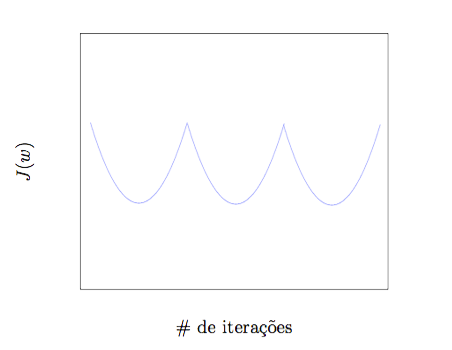
\includegraphics[scale=0.63]{figs/gd_multi_graph.png}
\label{f.gd_multi_graph}
\end{figure}

\subsection{Ferramentas Adicionais}
\label{s.additional_tools}

No caso de possuirmos espaços de características complexos, pode ser necessário empregar funções de regressão diferentes. Podemos utilizar, por exemplo, polinômios de grau 2:

\begin{equation}
\label{e.second_regression}
h_w(x) = w_0x_0 + w_1x_1 + w_2x^2.	
\end{equation}

Adicionalmente, é provável que os preços das casas comecem a estabilizar depois de um certo tamanho.

Considerando a regressão linear multivariável, ao invés de computar derivadas parciais para posterior computação do Gradiente Descendente, podemos resolver analiticamente a Equação~\ref{e.multi_optimization2}. Basicamente, podemos reescrever a Equação~\ref{e.multi_optimization2} como segue:

\begin{equation}
\label{e.multi_optimization3}
y_i = w^Tx_i, \forall i = 1, 2, \dots, m.
\end{equation}

Seja $X$ a matriz contendo todas as amostras de treinamentos, por exemplo:

\[X=
  \begin{bmatrix}
    x_1^0 & x_1^1 & x_1^2 & \dots & x_1^n \\
    x_2^0 & x_2^1 & x_2^2 & \dots & x_2^n \\
    \vdots & \ddots & & & \vdots \\
    x_m^0 & x_m^1 & x_m^2 & \dots & x_m^n \\
  \end{bmatrix}, \in \mathbb{R}^{m\times (n+1)}\] \\

Adicionalmente, seja $Y$ a matriz contendo todos os preços reais, por exemplo: 

\[Y=
  \begin{bmatrix}
    y_1 \\
    y_2 \\
    \vdots \\
    y_m
  \end{bmatrix}, \in \mathbb{R}^{m\times1}\] \\
  
Podemos reescrever a Equação~\ref{e.multi_optimization3} considerando todos os pontos dos dados de treinamento como segue:
  
\begin{equation}
\label{e.linear_system}
Y = w^TX.	
\end{equation}

Como podemos observar, a equação acima modela um sistema linear, que pode ser solucionado como segue:

\begin{equation}
\label{e.solution_linear_system}
w = (X^TX)^{-1}X^TY,
\end{equation}

onde $A^{-1}$ é o inverso da matriz $A = X^TX$. Em suma, podemos sumarizar os seguintes pontos para cada técnica:

\begin{itemize}
\item \textbf{Gradiente Descendente:} necessita da escolha de $alpha$, necessita várias iterações, funciona muito bem até para $n \rightarrow \infty$;
\item \textbf{Equação:} não necessita da escolha de $\alpha$, não necessita iterar, necessita computar $(X^TX)^{-1}$, o qual pode ser lento quando $n \rightarrow \infty$.
\end{itemize} 
\section{Regressão Logística}
\label{s.logistic_regression}

\subsection{Problemas de duas classes}
\label{ss.twoclass_problem}

Suponha que tenhamos um problema de classificação binária (i.e. um problema de duas classes, $y \in \{0,1\}$). Uma simples ilustração desse problema é dada a seguir:

 \begin{center}
 	\begin{tikzpicture}[domain=0:1]
  	\begin{axis}[ 
    	xlabel=Tamanho do tumor,
    	ylabel={Maligno?}
  		] 
    	\addplot[blue, thick] {x}; 
    	\addplot[only marks, red] plot coordinates {
        (0.3,1)
        (0.4,1) 
        (0.5,1)
        (0.9,1)
        (0.1,0)
        (0.2,0) 
        (0.3,0)
        (0.4,0)      
    };
  	\end{axis}
	\end{tikzpicture}
 \end{center}
 
Podemos utilizar uma regressão linear aqui, com a seguinte regra:\\se $(h_w(x) > 0.5)$ $y =$ SIM, se não $y =$ NÃO.
 
Entretanto, pode-se ter conjuntos de treinamentos mais complexos. Em tais casos, a Regressão Linear pode não ser plausível para solucionar o problema, como segue:
 
  \begin{center}
 	\begin{tikzpicture}[domain=0:1]
  	\begin{axis}[ 
    	xlabel=Tamanho do tumor,
    	ylabel={Maligno?}
  		] 
    	\addplot[blue, thick] {x - 1}; 
    	\addplot[only marks, red] plot coordinates {
        (-0.1,-1)
        (0.1,-1)
        (0.2,-1) 
        (0.3,-1)
        (0.4,-1)      
    };
        \addplot[only marks, black] plot coordinates {
        (0.3,1)
        (0.4,1) 
        (0.5,1)
        (0.9,1)
    };
  	\end{axis}
	\end{tikzpicture}
 \end{center}
 
Portanto, mesmo quando sabemos que a saída de nosso problema é 0 ou 1, é estranho que $h_w(x)$ possa assumir valores $> 1$ ou $< 0$. Tal como, se sabemos que nossa saída está no intervalo $h_w(x) \in [0,1]$, podemos aplicar a \textbf{Regressão Logística} para tal caso. Embora seja chamado de Regressão Logística, ela é uma técnica de \textbf{classificação}.\\
 
\textbf{Modelo da Regressão Logística}\\

\begin{center}
 \begin{tikzpicture}
    \begin{axis}[
    	legend pos=north west,
        axis x line=middle,
        axis y line=middle,
        xmin=-1,
        xmax= 1,
        ymin= 0,
        ymax= 1,
        xlabel=$z$,
        ylabel=$g(z)$,
        tick align=outside,
        enlargelimits=false]
      \addplot[domain=-1:1, red, ultra thick,samples=500] {1/(1+exp(-5*x))};
    \end{axis}
 \end{tikzpicture}
\end{center}
 
Queremos $0 \leq h_w(x) \leq 1$, com $h_w(x) = g(w^Tx)$, onde $g(z) = \frac{1}{1 + e^-z}$.
 
Portanto, temos que:

\begin{equation}
h_w(x) = \frac{1}{1 + e^{-w^Tx}}. 	
\end{equation}

Basicamente, a técnica de Regressão Logística tem por objetivo estimar $w$. Podemos interpretar a saída de hipótese como segue:

\begin{equation}
h_w(x) = P(y = 1 \mid x; w),
\end{equation}

onde significa a probabilidade de $y = 1$ dado $x$ parametrizado por $w$.

\begin{center}
 \begin{tikzpicture}
    \begin{axis}[
    	legend pos=north west,
        axis x line=middle,
        axis y line=middle,
        xmin=-1,
        xmax= 1,
        ymin= 0,
        ymax= 1,
        xlabel=$z$,
        ylabel=$g(z)$,
        tick align=outside,
        enlargelimits=false]
      \addplot[domain=-1:1, red, ultra thick,samples=500] {1/(1+exp(-5*x))};
    \end{axis}
 \end{tikzpicture}
\end{center}

\begin{center}
$g(z) \geq 0.5$ quando $z \geq 0$\\
$h_w(x) = g(w^Tx) \geq 0$ quando $w^Tx \geq 0$\\
$h_w(x) = g(w^Tx) < 0$ quando $w^Tx < 0$\\	
\end{center}

Suponha que tenhamos a seguinte situação:

\begin{center}
 \begin{tikzpicture}
    \begin{axis}[
    	legend pos=north west,
        axis x line=middle,
        axis y line=middle,
        xmin=-1,
        xmax= 4,
        ymin= -1,
        ymax= 4,
        xlabel=$x_1$,
        ylabel=$x_2$,
        tick align=outside,
        enlargelimits=false]
      \addplot[domain=-4:4, red, ultra thick,samples=500] {-x + 3};
      \addplot[only marks, blue] plot coordinates {
        (0.1,1)
        (0.3,1) 
        (0.5,1)
        (0.7,1) 
        (0.1,1.25)
        (0.3,1.25) 
        (0.5,1.25)
        (0.7,1.25)      
    };
        \addplot[only marks, black] plot coordinates {
        (2.9,1.5)
        (2.7,1.5) 
        (2.5,1.5)
        (2.3,1.5)
        (2.9,1.75)
        (2.7,1.75) 
        (3.1,1.75)
        (3.3,1.75)
        (3.7,2)
        (3.5,2) 
        (3.3,2)
        (3.1,2)
    };
    \end{axis}
 \end{tikzpicture}
\end{center}

\begin{center}
$x_1 + x_2 = 3$ (LIMITE DE DECISÃO), corresponde a $h_w(x) = 0.5$\\
$h_w(x) = g(w^Tx) = g(w_0 + w_1x_1 + w_2x_2)$, onde \[W=
  \begin{bmatrix}
    -3 \\
    1 \\
    1 
  \end{bmatrix}\]
\end{center}

Portanto, queremos prever $y = 1$ se $-3 + x_1 + x_2 \geq 0 \Rightarrow x_1 + x_2 \geq 3$.\\

\textcolor{red}{OBS: Falta exemplo do círculo.} \\

Vamos sumarizar o nosso problema:\\

\textbf{conjunto de treinamento:} $X = \{(x_1, y_1), (x_2, y_2), \dots, (x_m, y_m)\}$, $x_i \in \mathbb{R}^{n+1} \Rightarrow x_i^0 = 1$, $y_i \in \{0, 1\}$\\

\textbf{função de hipótese:} $h_w(x) = \frac{1}{1 + e^{w^Tx}}$

Como escolher parâmetros?\\

\textbf{função de custo:} $J(w) = \frac{1}{m} \sum_{i=1}^{m} (h_w(x_i) - y_i)^2$

Entretanto, como $h_w(x)$ agora é não linear, podemos ter uma função de custo não convexa, portanto há a necessidade de utilizar outra função de custo.\\

Seja $custo(h_w(x), y) = (h_w(x) - y)^2$ (MSE). Agora, devemos utilizar uma função de custo diferente:

\begin{equation}
\label{e.new_cost_function}
custo(h_x(x), y) = 
   \begin{cases}
      -log(h_w(x)), & \text{se}\ y=1 \\
      -log(1 - h_w(x)), & \text{se}\ y=0.
    \end{cases}
\end{equation}\\


 \begin{center}
 	\begin{tikzpicture}[domain=0:1]
  	\begin{axis}[ 
    	xlabel=$w$,
    	ylabel={$J(w)$, se $(y = 1)$},
    	ytick=\empty,
    	xtick=\empty
  		] 
    	\addplot[blue, thick] {-ln(x)};
  	\end{axis}
	\end{tikzpicture}
 \end{center}
 
\noindent Se $y = 1$ e $h_w(x) = 1$, então $custo(h_w(x), y) = 0$ (CORRETO).\\
Se $y = 1$ e $h_w(x) = 0$, então $custo(h_w(x), y) = \infty$ (ERRADO).
 
  \begin{center}
 	\begin{tikzpicture}[domain=0:0.8]
  	\begin{axis}[ 
    	xlabel=$w$,
    	ylabel={$J(w)$, se $(y = 0)$},
    	ytick=\empty,
    	xtick=\empty
  		] 
    	\addplot[blue, thick] {-ln(1-x)};
  	\end{axis}
	\end{tikzpicture}
 \end{center}
 
\noindent Se $y = 0$ e $h_w(x) = 0$, então $custo(h_w(x), y) = -log(1-0) = -log(1) = 0$ (CORRETO).\\
Se $y = 0$ e $h_w(x) = 1$, então $custo(h_w(x), y) = -log(1-1) = -log(0) = \infty$ (ERRADO).\\

Podemos reescrever a Equação~\ref{e.new_cost_function} como segue:

\begin{equation}
\label{e.newnew_cost_function}
custo(h_w(x), y) = -y log(h_w(x)) - (1 - y) log(1 - h_w(x)).	
\end{equation}

Portanto, a função de custo geral (todo conjunto de treinamento) considerando a técnica de Regressão Logística pode ser dada por:

\begin{equation}
\label{e.general_cost_function}
J(w) = \frac{1}{m} \sum\limits_{i=1}^m custo(h_w(x_i), y_i)
\end{equation}
\begin{center}
$= \frac{-1}{m} [\sum\limits_{i=1}^m y_i log(h_w(x_i)) + (1 - y_1) log(1 - h_w(x_i))]$		
\end{center}


Novamente, temos o seguinte problema de minimização: $min_{w} \quad J(w)$.

Podemos solucionar o seguinte problema de optimização:\\

 repita até convergência \{ \\ \\
 \hspace*{25pt} $w_j \leftarrow w_j - \alpha \frac{\partial J(w)}{\partial w_j}$ \\ \\
 \hspace*{15pt} \}\\
 
Temos que:
 
\begin{equation}
\alpha \frac{\partial J(w)}{\partial w_j} = \frac{1}{m} \sum\limits_{i=1}^m (h_w(x_i) - y_i)x^j
\end{equation}

Então, o algoritmo do Gradiente Descendente é dado por:\\
 
repita até convergência \{ \\ \\
 \hspace*{25pt} $w_j \leftarrow w_j - \alpha(\sum\limits_{i=1}^m(h_w(x_i) - y_i)x_i^j$ \\ \\
 \hspace*{15pt} \}
 
\subsection{Problema de múltiplas classes}
\label{ss.multiclass_problem}

A ideia da classificação de múltiplas classes é considerar o problema de aprender um espaço de características de $C$ classes, como segue:

 \begin{center}
 	\begin{tikzpicture}[domain=0:1]
  	\begin{axis}[ 
    	xlabel=$x_1$,
    	ylabel=$x_2$,
    	xtick=\empty,
    	ytick=\empty
  		] 
    	\addplot[only marks, red] plot coordinates {
        (0.15,0.1)
        (0.17,0.1) 
        (0.19,0.2)
        (0.21,0.2)      
    };
        \addplot[only marks, black] plot coordinates {
        (0.63,0.9)
        (0.65,0.9) 
        (0.67,1)
        (0.69,1)
    };
        \addplot[only marks, blue] plot coordinates {
        (0.45,0.5)
        (0.47,0.5) 
        (0.49,0.55)
        (0.51,0.55)
    };
  	\end{axis}
	\end{tikzpicture}\\
$y = \{0, 1, \dots, C - 1\}$
 \end{center}
 
Para lidar com tal problema, podemos considerar a abordagem \textbf{um-contra-todos} (\emph{one-versus-all} - OVA). Basicamente, se temos um problema de classificação de $C$-classes, podemos mapeá-lo em um problema de classificação de $C$-duas classes.

Portanto, temos a seguinte regra de decisão:

\begin{equation}
\label{e.decision_rule_logistic}
max_i \quad h_w^i(x) = P(y = 1 \mid x; w), \forall i = 1, 2, 3, \dots, C	
\end{equation}

Em suma, necessitamos treinar um classificador de regressão logística $h_w^i(x)$ para cada classe $i$ para prever o teste de probabilidade $y = i$. Em uma nova amostra de entrada $x$, podemos escolher sua classe $i$ como a qual maximiza a Equação~\ref{e.decision_rule_logistic}.
 
 
 








 

\section{Regularização}
\label{s.regularizacao}

\subsection{\emph{Overfitting}}
\label{ss.overfitting}

Voltemos ao problema de predizer os preços das casas considerando os seguintes exemplos:

  \begin{center}
 	\begin{tikzpicture}[domain=0:3]
  	\begin{axis}[ 
    	xlabel={Tamanho},
    	ylabel={Preço}
  		] 
    	\addplot[blue, thick] {x}; 
    	\addplot[only marks, red] plot coordinates {
        (0.5,0.5)
        (0.9,1)
        (1, 1)
        (0.8,1.2)
        (1.25, 1.15)
        (1.4, 1.2)
        (1.3, 1.5)
        (1.75, 1.85)
        (2, 2)
        (2.5, 2.3)
        (2.6, 2.8)
        
    };
  	\end{axis}
	\end{tikzpicture}
 \end{center}

Podemos perceber que o preço das casas pode não crescer linearmente. Dentro desse espectro de linearidade, nosso modelo pode subtreinar os dados de treinamento.

   \begin{center}
 	\begin{tikzpicture}[domain=-3:3]
  	\begin{axis}[ 
    	xlabel=Tamanho,
    	ylabel={Preço}
  		] 
    	\addplot[blue, thick] {sin(x^5)};
    	\addplot[only marks, red] plot coordinates {
        (-2.47, -1)
        (-1.3, -0.07)
        (0, 0)
        (1, 0.01)
        (1.93, 0.5)
        (2.45, 1)
        (2.9, -0.5)};
  	\end{axis}
	\end{tikzpicture}
 \end{center}

A função tenta "passar" (adaptar) através de todas as amostras de treinamento, causando o problema de supertreinamento (modelo muito específico).

Portanto, se tivermos muitas características, a hipótese aprendida pode acomodar bem os dados de treinamento ($J(w) \approx 0$), mas também pode falhar em generalizar novos exemplos (predizer os preços de novas casas).

Como podemos checar se tal situação ocorre ou não em nosso modelo? Se tivermos apenas duas características, podemos apenas visualizar o espaço de características. Caso contrário, podemos tentar realizar o seguinte:

\begin{itemize}

\item reduzir a quantidade de características (pode não ser a melhor ideia);
\item regularização: manter todas as características, mas reduzindo os valores dos parâmetros $w_j$ (funciona bem quando possuímos muitas características).
	
\end{itemize}

Suponha que penalizemos e fazemos $w_3$ e $w_4$ muito pequenos:

\begin{equation}
\label{e.small_w}
min_w \frac{1}{2m} \sum\limits_{i=1}^m (h_w(x_i) - y_i)^2 + 1000w_3 + 1000w_4.	
\end{equation}

Com isso, temos que $w_3$ e $w_4 \approx 0$. Na equação acima, se quisermos abrandar a influência de $w_3$ e $w_4$, podemos multiplicá-los por um valor alto (por exemplo $1000$). Basicamente, a ideia é ter valores \textbf{pequenos} para $w = (w_0, w_1, w_2, \dots, w_n)$ para ter uma função de hipótese mais simples (suave).

Basicamente, podemos pegar nossa função de custo (Equação~\ref{eq.mse}) e adicionar um segundo termo à ela, como segue:

\begin{equation}
\label{eq.mse_new}
J(w) = \frac{1}{2m} [\sum\limits_{i=1}^m (h_w(x_i) - y_i)^2 + \lambda\sum\limits_{j=1}^n w_j^2],
\end{equation}

onde $\lambda$ é o parâmetro de regularização que controla a relação entre a não regularização ($\lambda = 0$) e a regularização ($\lambda = \infty$).

\subsection{Regressão Linear Regularizada}
\label{ss.linear_regression_reg}

Nesta seção, iremos discutir sobre a regularização na abordagem de regressão linear. Novamente, nossa ideia é minimizar a Equação~\ref{eq.mse_new}, ou seja, encontrar $w$ o qual minimiza $J(w)$.

Portanto, podemos reescrever o algoritmo do Gradiente Descendente a fim de considerar a Equação~\ref{eq.mse_new} como segue:\\

 repita até convergência \{ \\ \\
 \hspace*{25pt} $w_0 \leftarrow w_0 - \alpha \frac{1}{m} \sum_{i=1}^{m}(h_w(x_i) - y_i) x_i^0$ \\~\\
 \hspace*{25pt} $w_j \leftarrow w_j - \alpha [\frac{1}{m} \sum_{i=1}^{m}(h_w(x_i) - y_i)x_i^j + \frac{\lambda}{m}w_j]$ \\ \\
 \hspace*{15pt} \}\\

Podemos generalizar o problema para uma formulação matricial também:

\[X=
  \begin{bmatrix}
    x_1^0 & x_1^1 & x_1^2 & \dots & x_1^n \\
    x_2^0 & x_2^1 & x_2^2 & \dots & x_2^n \\
    \vdots & \ddots & & & \vdots \\
    x_m^0 & x_m^1 & x_m^2 & \dots & x_m^n \\
  \end{bmatrix}, \in \mathbb{R}^{m\times (n+1)}\] \\
  
\[Y=
  \begin{bmatrix}
    y_1 \\
    y_2 \\
    \vdots \\
    y_m
  \end{bmatrix}, \in \mathbb{R}^{m\times1}\] \\
  
Podemos reescrever a Equação~\ref{e.solution_linear_system} a fim de considerar o termo de regularização:

\begin{equation}
w = (X^TX + \lambda A)^{-1} X^TY
\end{equation}

onde $A$ é uma matriz $(n+1)\times(n+1)$, como segue:

\[A=
  \begin{bmatrix}
    0 & 0 & 0 & \dots & 0 \\
    0 & 1 & 0 & \dots & 0 \\
    0 & 0 & 1 & \dots & 0 \\
    \vdots & & & \ddots & \vdots \\
    0 & 0 & 0 & \dots & 1 \\
  \end{bmatrix}, \in \mathbb{R}^{m\times (n+1)}\] \\
  
\textbf{Exemplo para $n = 2$:}

\[A=
  \begin{bmatrix}
    0 & 0 & 0 \\
    0 & 1 & 0 \\
    0 & 0 & 1 \\
  \end{bmatrix}\] \\
  
A razão para tal situação é garantir que $(X^TX + \lambda A)^{-1}$ seja inversível.

\subsection{Regressão Logística Regularizada}
\label{ss.logistic_regression_reg}

Nesta seção, iremos discutir sobre o classificador de Regressão Logística com o termo de regularização. Podemos reescrever a Equação~\ref{e.general_cost_function} como segue:

\begin{equation}
\label{e.log_regression_new}
-1[\frac{1}{m} [\sum\limits_{i=1}^m y_i log(h_w(x_i)) + (1 - y_1) log(1 - h_w(x_i))]	 + \frac{\lambda}{2m} \sum\limits_{j=1}^n w_j^2.
\end{equation}

Podemos implementar a equação acima considerando o Gradiente Descendente:\\

repita até convergência \{ \\ \\
 \hspace*{25pt} $w_0 \leftarrow w_0 - \alpha(\sum\limits_{i=1}^m(h_w(x_i) - y_i)x_i^0$ \\ \\
 \hspace*{25pt} $w_j \leftarrow w_j - \alpha(\sum\limits_{i=1}^m(h_w(x_i) - y_i)x_i^j + \frac{\lambda}{m}w_j$ \\ \\
 \hspace*{15pt} \}
 

\section{Redes Neurais}
\label{s.neural_networks}

\subsection{Neurônios e o Cérebro}

Nesta seção, vamos discutir sobre os princípios das redes neurais. Tais técnicas tentam imitar o cérebro humano, sendo vastamente utilizadas nas décadas de 80 e 90. Com o surgimento de novas ferramentas por volta do meio da década de 90, sua popularidade acabou por decrescer. Entretanto, elas voltaram a ter um foco maior devido às abordagens baseadas em aprendizado em profundidade. Segue um exemplo de um simples neurônio:

\begin{figure}[!h]
\centering
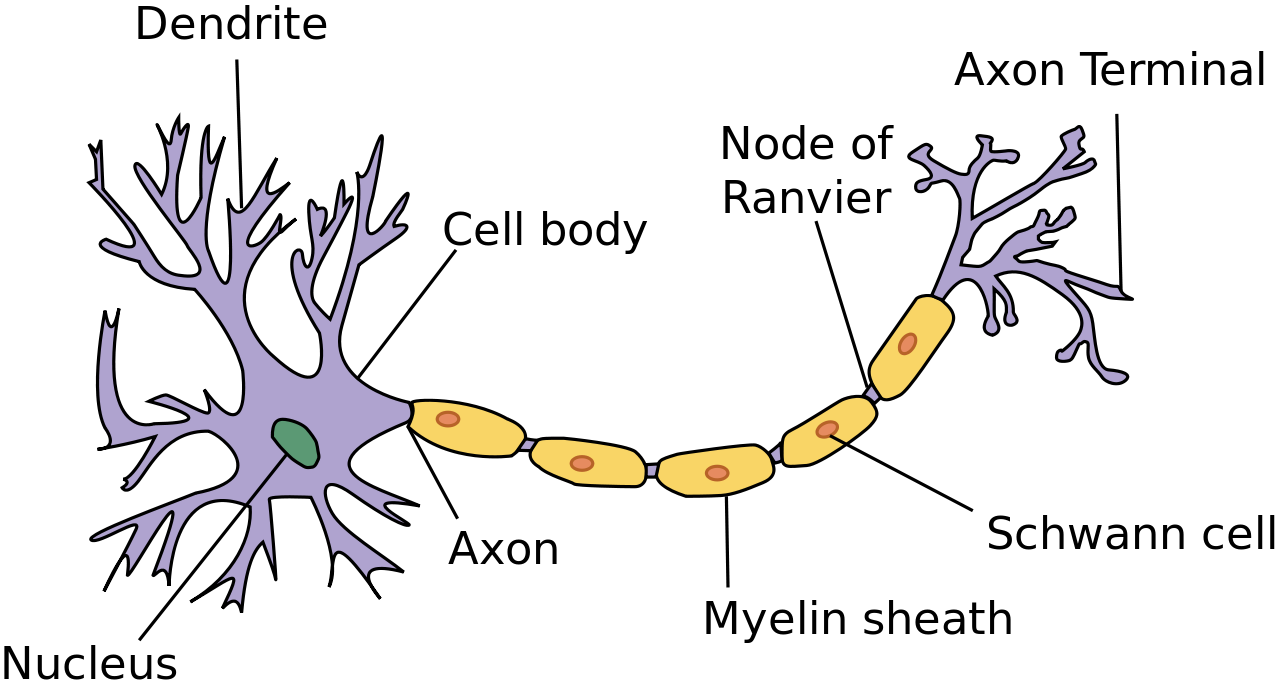
\includegraphics[scale=0.25]{figs/neuron.png}
\label{f.neuron}
\end{figure}

Basicamente, os neurônios comunicam entre si por meio da emissão de pulsos elétricos a partir de suas entradas (dendrito) para suas saídas (axônio). Matematicamente falando, podemos representar um simples neurônio como segue:

\begin{figure}[!h]
\centering
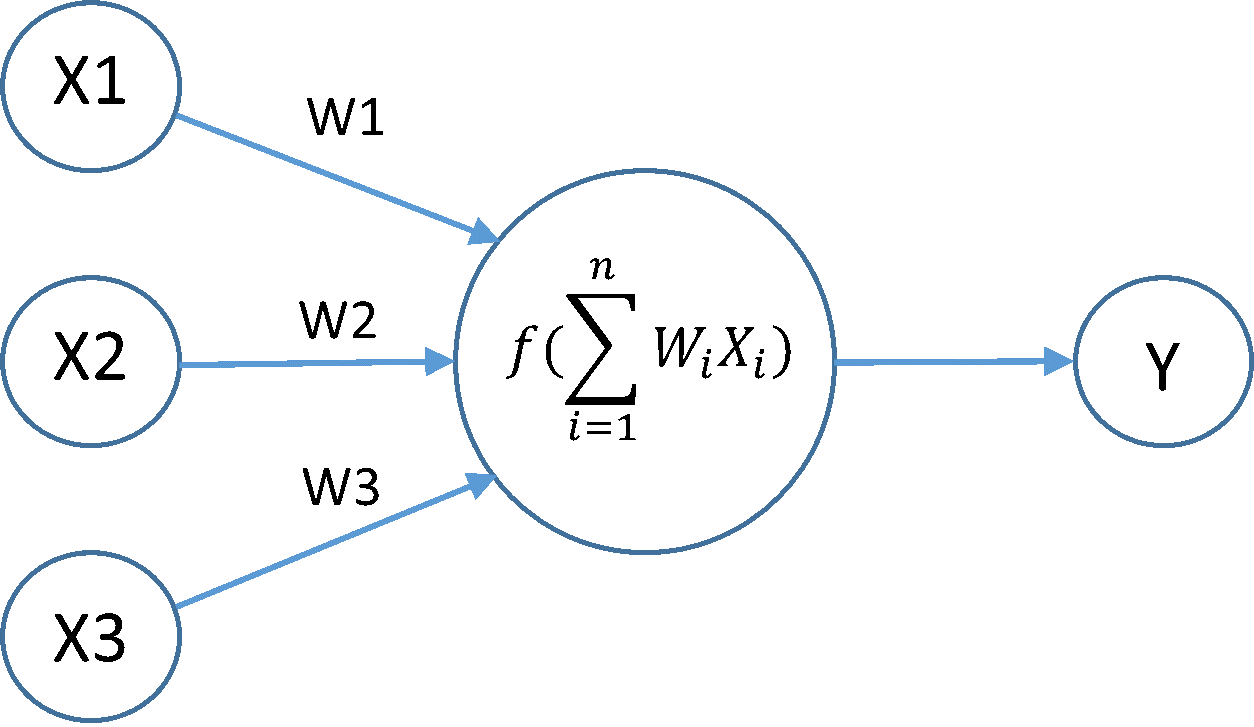
\includegraphics[scale=0.30]{figs/simple_neural_network.png}
\label{f.simples_neural_network}
\end{figure}

Uma \textbf{função de ativação} comum que pode ser utilizada é:

\begin{equation}
\label{e.activation_function}
g(z) = \frac{1}{1 + e^{-z}}, \text{onde} \ z = w^Tx	
\end{equation}

ou uma função limiar:

\begin{equation}
\label{e.limiar_function}
g(z) =
   \begin{cases}
      1, & \text{if}\ z \geq \theta \\
      0, & \text{se}\ z < \theta,
    \end{cases}
\end{equation}

onde $\theta$ é um limite dado.

A equação acima pode ser reescrita como segue:

\begin{equation}
\label{e.limiar_function_r}
h_w(x) =
   \begin{cases}
      1, & \text{se}\ w^Tx \geq \theta \\
      0, & \text{se}\ w^Tx < \theta.
    \end{cases}
\end{equation}

\subsection{Perceptron}
\label{ss.perceptron}

O Perceptron foi proposto formalmente por McCulloch e Pitts em 1943 com o intuito de modelar um neurônio biológico. Entretanto, ele possui uma capacidade limitada em termos de poder discriminativo, dado que ele é capaz de aprender apenas um único hiperplano.

Novamente, vamos considerar nosso conjunto de treinamento $X = \{(x_0, y_0), (x_1, y_1), \dots, (x_n, y_n)\}$, onde $x_i \in \mathbb{R}$ e $y_i \in \{0, 1\}$. Para uma dada amostra $x \in X$, temos a seguinte situação:

\begin{table}[h]
\centering
\begin{tabular}{c|c|c}
\hline
\textbf{\small Rótulo Verdadeiro $(y)$} & \textbf{\small Rótulo Proposto $h_w(x)$} & \textbf{Erro} $\epsilon$\\\hline \hline
{\small 0} & {\small 0} & {\small 0}\\\hline
{\small 1} & {\small 0} & {\small 1}\\\hline
{\small 0} & {\small 1} & {\small -1}\\\hline
{\small 1} & {\small 1} & {\small 0}\\\hline
\end{tabular}
\label{t.perceptron}
\end{table}

Podemos reescrever a função de ativação limiar como segue:

\begin{equation}
\label{e.limiar_function_r1}
h_w(x) =
   \begin{cases}
      1, & \text{se}\ w^Tx - \theta \geq 0 \\
      0, & \text{se}\ w^Tx  - \theta < 0.
    \end{cases}
\end{equation}

Se considerarmos $w_0 = -\theta$, então temos:

\begin{equation}
\label{e.limiar_function_r2}
h_w(x) =
   \begin{cases}
      1, & \text{se}\ w^Tx \geq 0 \\
      0, & \text{se}\ w^Tx < 0.
    \end{cases}
\end{equation}

Antes de aprender o mecanismo de funcionamento do Perceptron, temos que compreender alguns conceitos relacionados à projeções e produtos internos. Suponha que tenhamos dois vetores $w = [w_1 w_2]$ e $x = [x1 x2]$. Podemos definir o seu produto interno (vetorial) entre $w$ e $x$ como: $w^Tx$. Podemos visualizar tal ideia como segue:

\begin{equation}
\parallel w \parallel = \sqrt{w_i^2 + w_2^2} \in \mathbb{R} \Rightarrow \text{tamanho (norma) do vetor} \ w	
\end{equation}

E o produto interno pode ser representado como segue:

\begin{center}
$p =$ tamanho da projeção de $w$ em $x$.
\end{center}

Portanto, $w^Tx = p \parallel w \parallel$.\\

Consideremos a situação onde $y = 1$ e $h_w(x) = 0$. Neste caso, $\epsilon = (y - h_w(x)) = (1 - 0) = 1$ (erro). Dado $h_w(x) = 0$, então temos que $w^Tx < 0$ (função de ativação limiar).

Também temos que $w^Tx < 0$ significa $p \parallel w \parallel \Rightarrow p < 0$. Entretanto, necessitamos $h_w(x) = 1$ para acertar a classificação. A fim de se obter isto, é desejável mover $w^{(t)}$ em direção à $x$, onde $w^{(t)}$ significa o valor de $w$ na iteração $t$.

Nesta situação, podemos obter $w^{(t + 1)}$ como segue: $w^{(t + 1)} = w^{(t)} + \eta x$, onde $\eta$ é a taxa de aprendizado.

Agora, suponha outra situação, onde $y = 0$ e $h_w(x) = 1$. Neste caso, temos que $\epsilon = (y - h_w(x)) = (0 - 1) = -1$ (erro). Portanto, temos que $w^Tx \geq 0$, mas necessitamos $w^Tx < 0$ dado que $y = 0$.

Portanto, podemos computar $w^{(t + 1)}$ como segue: $w^{(t + 1)} = w^{(t)} - \eta x$. Podemos juntar as duas equações em somente uma:

\begin{equation}
w^{(t + 1)} = w^{(t)} + \eta \epsilon x, \text{onde} \ \epsilon \in \{-1, 0, 1\}.
\end{equation}\\

Finalmente, o algoritmo de treinamento do perceptron é dado como segue:

\begin{enumerate}
\item Inicializar $\eta$;
\item Inicializar $w$ (pesos aleatórios);
\item Aplicar $w^{(t + 1)} = w^{(t)} + \eta \epsilon_i x_i, \forall i = 1, 2, \dots, m$ e $\epsilon_i(y_i - h_w(x+i))$;
\item Repetir passo (3) até que $\epsilon_i = 0$ para todos os elementos em $X$.
\end{enumerate}

\subsection{Perceptron Multi-camadas}
\label{ss.multi_perceptron}

Uma rede neural é basicamente um grupo de neurônios, como segue:

\begin{figure}[!h]
\centering
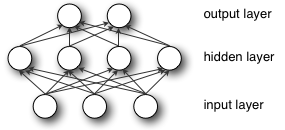
\includegraphics[scale=0.75]{figs/mlp.png}
\label{f.mlp}
\end{figure}

Considerando a rede acima, temos:

\begin{center}
$a_1^{(2)} = g(w_{01}^{(1)} x_0 + w_{11}^{(1)} x_1 + \dots + w_{n1} x^n)$
\\~\\
$a_2^{(2)} = g(w_{02}^{(1)} x_0 + w_{12}^{(1)} x_1 + \dots + w_{n2} x^n)$
\\~\\
$h_w(x) = a_1^{(3)} = g(w_{01}^{(2)} a_0^{(2)} + w_{11}^{(1)} a_1^{(2)} + w_{21}^{(2)} a_2^{(2)})$
\end{center}

Podemos também representar a rede neural como uma matriz de elementos como segue:

\[X=
  \begin{bmatrix}
    x^0 \\
    x^1 \\
    x^2 \\
    \vdots \\
    x^n
  \end{bmatrix}\]
  
\[Z^{(2)}=
  \begin{bmatrix}
    z_0^{(2)} \\
    z_1^{(2)} \\
    z_2^{(2)} \\
  \end{bmatrix} = (w^{(1)})^T X\]
  
\begin{center}
$a^{(2)} = g(z^{(2)} \Rightarrow h_w(x) = a^{(3)} = g(z^{(3)}$
\\~\\
$z^{(3)} = (w^{(2)})^Ta^{(2)}$
\end{center}

$Z_i^{(k)}$ refere-se aos dados de entrada do neurônio $i$ da camada $k$. Note que o processo computacional das ativações das unidades de entrada, escondida e saída é chamado de \emph{forward propagation}.

Se tivermos um problema de classificação de múltiplas classes, então o número de saída de neurônios será o mesmo que o número de classes.

Suponha que tenhamos um problema com $3$ classes. Portanto, $h_w(x) \in \mathbb{R}$. Considerando o problema, cada unidade de saída é composta por 3 classificadores de regressão logística.

\subsection{Parâmetros de Aprendizado}
\label{ss.learning_parameters}

Agora, a próxima questão é: como podemos aprender o conjunto de parâmetros $w = (w^{(1)}, w^{(2)}, \dots, w^{(L-1)})$, onde $L$ é o número de camadas. Seja $s_l$ o número de neurônios na camada $l$ (não estamos considerando as unidades de \emph{bias}).

Vamos rever a função de custo utilizada pela Regressão Logística.

\begin{equation}
\label{e.nn_costfunction}
J(w) = \frac{1}{m}[\sum\limits_{i=1}^m (y_i log(h_w(x_i)) + (1 - y_i) log(1 - h_w(x_i)))] + \frac{\lambda}{2m}\sum\limits_{j=1}^m w_j^2	
\end{equation}

Considerando uma rede neural com $k$ classes, então teremos $k$ classificadores de regressão logística na unidade de saída. Portanto, a função de custo deve considerar esses $k$ classificadores logísticos, como uma generalização da Equação~\ref{e.nn_costfunction}:

\begin{equation}
J(w) = \frac{-1}{m}[\sum\limits_{i=1}^m\sum\limits_{k=1}^k y_i^k log(h_w^k(x_i))+(1-y^k)log(1-h_w^k(x_i))] + \frac{\lambda}{2m}\sum\limits_{l=1}^{L-1}\sum\limits_{i=1}^{s_l}\sum\limits_{j=1}^{s_{l+1}}(w_{ij}^{(l)})^2
\end{equation}

Nosso próximo passo consiste em utilizar um conhecido algoritmo para o aprendizado de parâmetros em redes neurais chamado de \emph{Backpropagation}. Basicamente, queremos minimizar $J(w)$, e para tal propósito necessitamos computar as derivadas parciais $\frac{\partial J(w)}{\partial w_{ij}^{(l)}}$, onde $w_{ij}^{(0)} \in \mathbb{R}$.

Suponha que tenhamos apenas uma amostra de treinamento $(x, y)$ e a seguinte arquitetura de rede neural:

Os passos da \emph{forward propagation} são dados como segue:

\begin{itemize}
\item $a^{(1)} = x$
\item $z^{(2)} = (w^{(1)})^T a^{(1)}$
\item $a^{(2)} = g(z^{(2)})$
\item $z^{(3)} = (w^{(2)})^T a^{(2)}$
\item $a^{(3)} = g(z^{(3)})$
\item $z^{(4)} = (w^{(3)})^T a^{(3)}$
\item $a^{(4)} = h_w(x) = g(z^{(3)})$	
\end{itemize}

O propósito do algoritmo do \emph{Backpropagation} é relacionado ao cálculo do gradiente. Temos uma nova variável $\iota_j^{(l)}$ que significado o erro do nó $j$ na camada $l$.

Considerando a rede acima, temos que:

\begin{itemize}
\item para cada camada de saída $(l = 4)$: $\iota_j^{(4)} = a_j^{(4)} - y_j \Rightarrow \iota^{(4)} = a^{(4)} - y$	
\item para cada camada escondida $l \in \{2,3\}$:
	\begin{center}
	$\iota^{(3)} = (w^{(3)})^T \iota^{(4)} \ast g^1(z^{(3)})$
	\\~\\
	$\iota^{(2)} = (w^{(2)})^T \iota^{(3)} \ast g^1(z^{(2)})$
	\\~\\
	$\iota^{(l)} = (w^{(l)})^T \iota^{(l+1)} \ast g^1(z^{(l)})$
	\\~\\
	$g^1 = $ derivada da função de ativação
	\end{center}
\end{itemize}

\textbf{Ex.:} $g(z^{(3)}) = a^{(3)}$, $g^1(z^{(3)}) = a^{(3)} \ast (1 - a^{(3)})$\\

O nome \emph{Backpropagation} refere-se ao fato de que são computadas $\iota^{(4)}$, $\iota^{(3)}$ e $\iota^{(2)}$, o que significa que retropropagamos o erro através da rede. Basicamente, as derivadas parciais são dadas por:

\begin{equation}
\frac{\partial J(w)}{\partial W_{ij}^{(l)}} = a_i^{(l)} \iota_j^{(l+1)}	
\end{equation}

Note que não estamos considerando o termo de regularização.







\section{Máquinas de Vetores de Suporte}
\label{s.svm}

Com o intuito de obter os principais conceitos sobre as Máquinas de Vetores de Suporte (SVMs), podemos observar primeiramente o classificador de Regressão Logística, o qual será modificado para suprir nossas necessidades.

Novamente, temos a seguinte equação para descrever o classificador de Regressão Logística:

\begin{center}
$h_w(x)=\frac{1}{1+e^{-w^Tx}}$	
\end{center}

Se $(y = 1)$, queremos que $h_w(x) \approx 1 \Rightarrow w^Tx >> 0$.
Se $(y = 0)$, queremos que $h_w(x) \approx 0 \Rightarrow w^Tx << 0$.\\

Considerando a função de custo da Regressão Logística que já sabemos:

\begin{equation}
custo(h_w(x)) y = -(y log(h_w(x)) + (1-y)log(1-h_w(x))
\end{equation}
\begin{center}
$= -(y log \frac{1}{1+e^{-w^Tx}} + (1-y) log (1- \frac{1}{1+e^{-w^Tx}})$.
\end{center}

Note que a função de custo acima considera apenas uma amostra de treinamento. Olhemos a função de custo geral do classificador de Regressão Logística:

\begin{equation}
\label{e.svm_cost}
min_w \frac{1}{m} [\sum\limits_{i=1}^m y_i (-log(h_w(x_i)) + (1-y_i)(-log(1-h_w(x_i)))] + \frac{\lambda}{2m} \sum\limits_{j=1}^n w_j^2,
\end{equation}

a qual é basicamente a Equação~\ref{e.nn_costfunction}, mas com um sinal de ``$-$" dentro de cada termo.

Podemos reescrever a Equação~\ref{e.svm_cost} como segue:

\begin{equation}
\label{e.svm_newcost}
min_w \frac{1}{m}[\sum\limits_{i=1}^m y_i custo_1(w^Tx) + (1-y_i)custo_o(w^Tx)] + \frac{\lambda}{2m} \sum\limits_{j=1}^n w_j^2
\end{equation}

Entretanto, para considerar a formulação do SVM, é necessário reescrever a Equação~\ref{e.svm_newcost} como segue:

\begin{enumerate}
\item Vamos remover a constante $\frac{1}{m}$:\\
$min_w [\sum\limits_{i=1}^m y_i custo_1(w^Tx) + (1-y_i)custo_o(w^Tx)] + \frac{\lambda}{2m} \sum\limits_{j=1}^n w_j^2$
\item Agora, retiremos o termo de regularização na segunda parte da Equação~\ref{e.svm_newcost}, e adicionemos ao primeiro termo, o qual é nomeado agora de $C$. A otimização é mantida similar se $C = \frac{1}{\lambda}$. Portanto, temos a seguinte função de custo geral considerando SVM:

\begin{equation}
\label{e.svm_c}
min_w C \sum\limits_{i=1}^m[y_i custo_1(w^Tx) + (1-y_i)custo_0(w^Tx)]+\frac{1}{2} \sum\limits_{j=1}^n w_j^2
\end{equation}

Note que as SVMs não retornam as probabilidades como a Regressão Logística faz, mas retorna a classe $h_w(x) \in \{0, 1\}$ para uma dada amostra $x$:

\begin{equation}
\label{e.svm_classes}
h_w(x) =
   \begin{cases}
      1, & \text{se}\ w^Tx \geq 0 \\
      0, & \text{caso contrário}.
    \end{cases}
\end{equation}

Basicamente, a ideia agora é aprender $w$.
\end{enumerate}

Quando $C$ for muito grande, o primeiro termo da Equação~\ref{e.svm_c} tende a 0. Neste contexto, temos algo parecido com isso:

\begin{equation}
\label{e.svm_c_zero}
min \quad C \times 0 + \frac{1}{2}\sum\limits_{j=1}^n w_j^2
\end{equation}
\begin{center}
sujeito à $w^Tx_i >> 1$ se $(y_i = 1)$ ou $w^Tx_i << -1$ se $(y_i = 0)$.
\end{center}

Novamente, o problema de otimização refere-se à procura de parâmetros do hiperplano que melhor separam os dados. Portanto, as SVMs tentam encontrar o hiperplano com a margem \textbf{máxima}.\\

\textbf{Relembrando:}\\

$w^Tx = p \parallel w \parallel$, onde $p$ é o tamanho da projeção de $x$ em $w$. Sabemos que $\parallel w \parallel = \sqrt{\sum\limits_{j=1}^n w_j^2}$, a qual é a norma do vetor $w$. Podemos reescrever a Equação~\ref{e.svm_c_zero} como segue:

\begin{equation}
\label{e.svm_min}
min_w \quad \frac{1}{2} \parallel w \parallel^2
\end{equation}
\begin{center}
sujeito à $w^Tx_i >> 1$ se $(y_i = 1)$ ou $w^Tx_i << -1$ se $(y_i = 0)$.
\end{center}

Portanto, temos que $w^Tx_i = p_i \parallel w \parallel$. Podemos modificar a Equação~\ref{e.svm_min} como segue:

\begin{equation}
min_w \quad \frac{1}{2} \parallel w \parallel^2	
\end{equation}
\begin{center}
sujeito à $p_i \parallel w \parallel >> 1$ se $(y_i = 1)$ ou $p_i \parallel w \parallel << -1$ se $(y_i = 0)$.
\end{center}

A probabilidade $1$ leva à $\sum\limits_{i=1}^m p_i$ menor que a mesma soma considerando a possibilidade  $2$. Se $\sum\limits_{i=1}^m p_i$ for muito grande, $w$ necessita ser pequeno (lembre-se que estamos tentando minimizar $w$).

\subsection{Trabalhando com Núcleos}
\label{ss.svm_kernels}

Suponha que possamos representar o limite de decisão como segue:

\begin{equation}
\label{e.boundary_limit}
h_w(x) = w_0 + w_1l_1 + w_2l_2 + \dots\text{, onde } h_1 = x_1, h_2 = x_2, \dots
\end{equation}

A questão é: podemos encontrar melhores calores para $l_1, l_2, \dots$ de tal modo que o limite de decisão seja menos complexo? Suponha que tenhamos três marcações no espaço de características, por exemplo, $l_1, l_2$ e $l_3$. 

Para uma dada amostra $x$, podemos definir:

\begin{center}
$l_1 = similaridade(x,l_1) = exp(\frac{-\parallel x - l_1 \parallel}{2\sigma^2})$ \\	
$l_2 = similaridade(x,l_2) = exp(\frac{-\parallel x - l_2 \parallel}{2\sigma^2})$ \\	
$l_3 = similaridade(x,l_3) = exp(\frac{-\parallel x - l_3 \parallel}{2\sigma^2})$ \\	
\end{center}

Está função $K(x, l_i)$ é chamada de função do núcleo, ativada por uma função de base radial do tipo gaussiana. \\

\noindent Se $x \approx l_1 \Rightarrow l_1 = exp(\frac{-0}{2\sigma^2}) = 1$.
\\
Se $x$ estiver distante de $l_1 \Rightarrow l_1 = exp(\frac{-\infty}{2\sigma^2}) = 0$. \\

Novamente, suponha que tenhamos $y = 1$ quando $w_0 + w_1l_1 + w_2l_2 + w_3l_3 \geq 0$. Seja $w^T = [=0.5 \ 1 \ 1 \ 0]$, e considere duas amostras como $x_1$ e $x_2$:

\begin{itemize}
\item Para $x_1$: $l_1 \approx 1, l_2 \approx 0, l_3 \approx 0 \Rightarrow w_0 + w_1l_1 + w_2l_2 + w_3l_3 = 0.5 + 1 = 0.5 > 0$.
\item Para $x_2$: $l_1 \approx 0, l_2 \approx 0, l_3 \approx 0 \Rightarrow w_0 + w_1l_1 + w_2l_2 + w_3l_3 = 0.5 < 0$.
\end{itemize}
  
Basicamente, também vamos terminar com uma função de decisão complexa.

A principal ideia é escolher cada exemplo de treinamento como uma marcação. Portanto, se tivermos $m$ exemplos, deveremos ter $l_i = x_i, x = 1, 2, \dots, m$.

Então, dado uma exemplo $x$:

\begin{center}
$f_i = similaridade(x, l_i) \Rightarrow f^T = [f_0 \ f_1 \ \dots f_m]$.	
\end{center}

Portanto, $x_i \in \mathbb{R}^{m+1}$ será representado como $f^i = [f_0^i \ f_1^i \dots f_m^i] \ in \mathbb{R}^{m+1}$.

Em suma, considerando SVM com núcleos, temos:

\begin{itemize}
\item Hipótese: dado $x$, calcula características $f \in \mathbb{R}^{m+1}$. Predizer $y = 1$ se $w^Tf \geq 0$.
\end{itemize}

A etapa de treinamento consiste em solucionar o seguinte problema de minimização.

\begin{equation}
min_w \ C \sum\limits_{i=1}^m y_i \ custo_1 (w^Tf^i) + (1 - y_i) \ custo_0 (w^Tf^i) + \frac{1}{2} \sum\limits_{j=1}^m w_j^2
\end{equation}

O principal problema é escolher o parâmetro $C$, bem como os parâmetros do núcleo.
\section{Aprendizado Não-Supervisionado}
\label{s.unsupervised_learning}

Vimos nas aulas anteriores que, dado um conjunto de treinamento rotulado $X = \{(x_1, y_1), (x_2, y_2), \dots, (x_m, y_m)\}$, um algoritmo de aprendizado supervisionado tem por objetivo aprender um limite de decisão o qual melhor separa as amostras de diferentes classes.

Basicamente, a ideia principal é alimentar o algoritmo não-supervisionado com dados, com o intuito de encontrar padrões. Portanto, nossa base de dados é modelada como $X = \{x_1, x_2, \dots, x_m\}$. Como a ideia é encontrar agrupamentos contidos nos dados, as técnicas não-supervisionadas geralmente são denominadas de agrupamentos.

\subsection{K-médias}
\label{ss.kmeans}

O algoritmo do k-médias é um dos mais utilizados para a classificação não-supervisionada. Ele possui duas etapas principais:

\begin{itemize}
\item atribuição dos agrupamentos;
\item atualização dos centros.	
\end{itemize}

Basicamente, utilizando o número de agrupamentos (médias) como uma entrada ($k$), escolhemos aleatoriamente $k$ amostras. Após, cada amostra do conjunto de dados é associada ao seu vizinho mais próximo. Adicionalmente, podemos computar os novos centros baseados nos valores médios da amostra que pertence a cada agrupamento. O algoritmo termina de iterar quando os novos centros não mudam suas posições durante as iterações.

Quando os agrupamentos estão bem-separados, o algoritmo do k-médias deve funcionar muito bem. A maioria dos algoritmos supervisionados vistos são modelados por uma função a ser otimizada, assim como no caso do k-médias.

Seja $k$ o número de agrupamentos, $c_i$ o número do agrupamento para o qual $x_i$ foi atribuído, $\mu_k$ o centro do agrupamento $(x, \mu_k \in \mathbb{R}^n)$, e $\mu_{c_i}$ o centro do agrupamento para o qual $x_i$ foi atribuído. A função de otimização é dada por:

\begin{equation}
\label{e.kmeans_optimization}
J(c_1, c_2, \dots, c_m, \mu_1, \mu_2, \dots, \mu_k) = \frac{1}{m} \sum\limits_{i=1}^m \parallel x_i - \mu_{c_i} \parallel.	
\end{equation}

Portanto, a ideia é solucionar o seguinte problema:

\begin{equation}
min \ J(c_1, c_2, \dots, c_m, \mu_1, \mu_2, \dots, \mu_k).	
\end{equation}

O k-médias pode ser implementado como segue:\\

 \noindent inicialize aleatoriamente $k$ centros de agrupamentos $\mu_1, \mu_2, \dots, \mu_k \in \mathbb{R}^n$\\~\\
 repita até convergência\{ \\ \\
 \hspace*{25pt} para $i = 1$ até $n$\\~\\
 \hspace*{35pt} $c_i \leftarrow index \in \{1, 2, \dots, k\}$ do centro do agrupamento mais perto de $k_i$\\~\\
  \hspace*{25pt} para $i = 1$ até $k$\\~\\
  \hspace*{35pt} $u_i \leftarrow$ média de todos os pontos atribuídos ao agrupamento $i$\\ \\
 \hspace*{15pt} \} \\



  
\end{document}